

\section{Key Invariant on Correspondence Between Back-edges of SEquential and Pipelined Loops}
 Our key invariant defines a ``correspondence relation''
between the back-edges of the sequential and pipelined CCDFGs.
The relation can be informally paraphrased as
follows~\cite{disha-itp14}.

\begin{figure}[t!]
\begin{center}
\begin{tabular}{c}
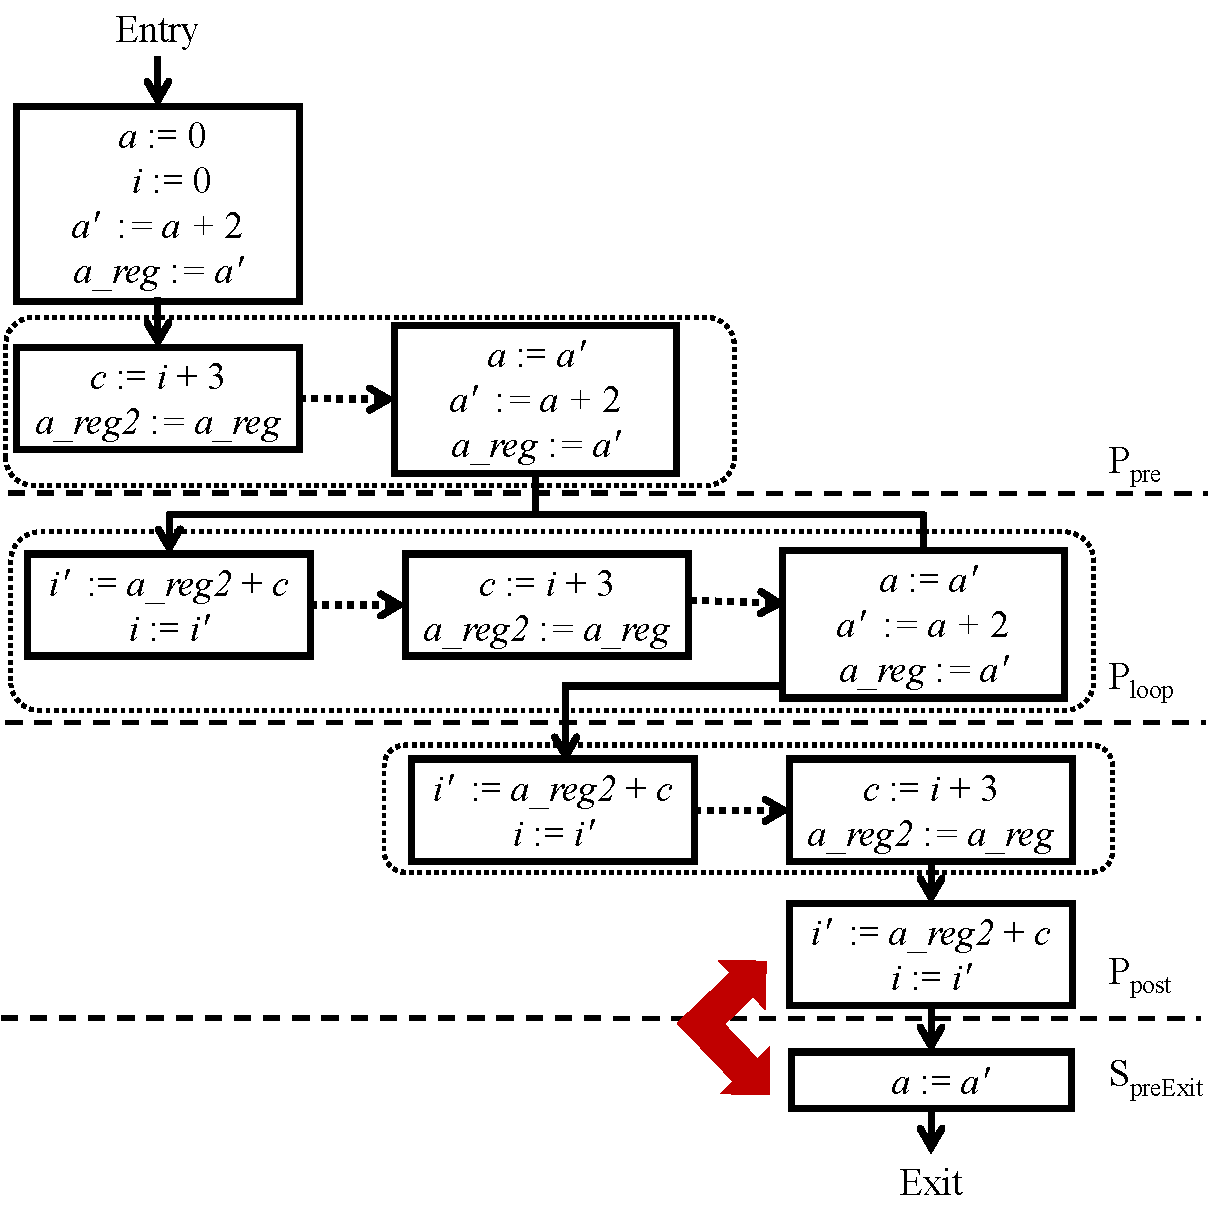
\includegraphics[width=5.5in]{fig-proposal/algorithm-after-superstep-construction}
\end{tabular}
\end{center}
\caption{Superstep Construction}
\label{fig:algo3-3}
\end{figure}

\begin{quote}
Let $S$ be a sequential loop and $P$ be the pipelined loop
generated from our algorithm. The pipelined loop after superstep construction
consists of
three stages before $S_{preExit}$ as depicted in
Figure~\ref{fig:algo3-3}: prologue $P_{pre}$, full stage
$P_{loop}$, and epilogue $P_{post}$.  Let $s_l$ be any state of $P$
poised to execute $P_{loop}$, and let $k$ be any number such that
the loop of $P$ is not exited in $k$ iterations from $s_l$.
Then executing $P_{pre}$ followed by $k$ iterations of $P_{loop}$ is
equivalent to executing first iteration of $S$, say $S_1$
followed by $(k - 1)$ iterations of $S$ together with a
collection of ``partially completed'' iterations of
$S$.\footnote{The formalization actually characterizes each
  incomplete iteration, \eg, if the pipeline includes $d$
  iterations and successive iterations are introduced in
  consecutive clock cycles, then the $i$-th iteration has $i
  - 1$ incomplete scheduling steps.}
\end{quote}

The partially completed iterations can be determined by the
length of the first iteration in $P_{pre}$ and the pipeline interval.
Suppose the length of the first iteration in $P_{pre}$
is {\tt m} and the pipeline interval is {\tt i}. Note that we
can calculate the value of {\tt m} based on the number of scheduling steps in a CCDFG
and the pipeline interval. The partially completed iterations mean $m$
scheduling steps of $S$ followed by $(m-i)$ scheduling steps of $S$, by
$(m-2i)$ scheduling steps of $S$, etc. while $(m-ni)$ is positive.

In our example, {\tt m} is $2$
and {\tt i} is $1$.  The invariant implies that starting
from the same initial state, executing $P_{pre}$ and {\tt k}
iterations of $P_{loop}$ is the same as executing {\em k}
iterations of $S$, followed by $m = 2$ scheduling steps of
$S$, followed by $ (m - i) = 1$ scheduling steps of $S$.

As is standard with proofs involving invariants, there are
two obligations to prove the correctness, \viz, that it is indeed
an invariant, and that its invariance is sufficient to imply
the desired correctness theorem.  Here we give a sense of
our envisioned proof.

The proof of invariance of this predicate is, of course, the
main ``work horse'' in this exercise.  The proof depends on
our interchange primitive which in turn is based on a fundamental idea for pipelining,
\viz, commutability of independent instructions.

\begin{quote}
Suppose that the
set of variables written and read by two consecutive
operations $a$ and $b$ is disjoint.  Then executing $a$
followed by $b$ generates the same result as executing $b$
followed by $a$.
\end{quote}

If we view the scheduling steps in
Figure~\ref{fig:invariant-base-case} as arranged in a
matrix, then the sequential execution proceeds column-wise
along the matrix while the pipelined execution proceeds
row-wise.  Thus the core proof obligation involves the
following two proof requirements.

\begin{enumerate}[--]
\item Our pipelining algorithm correctly combines the
  ``appropriate'' scheduling supersteps which do not have
  read-write hazards.
\item Given that there are no read-write hazards at
  appropriate places, executing scheduling steps row-wise is
  same as executing those scheduling steps column-wise in
  the pipelined CCDFG.  This requires the use of interchange primitive.
\end{enumerate}

\begin{figure}[t!]
\begin{center}
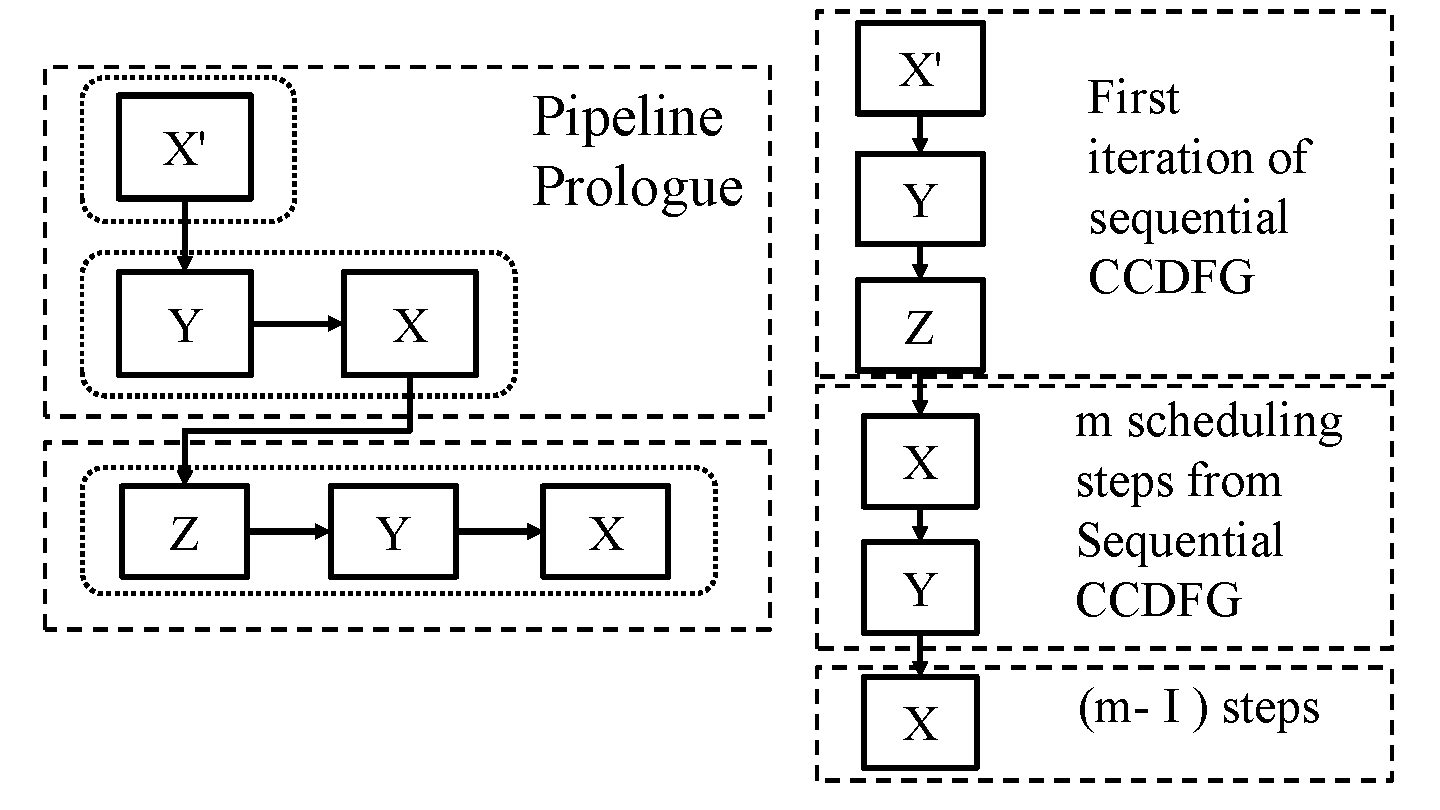
\includegraphics[width=4.25in]{fig-proposal/invariant-base-case}
\end{center}
\caption{Invariant base case where k = 1}
\label{fig:invariant-base-case}
\end{figure}

\begin{figure}[t!]
\begin{center}
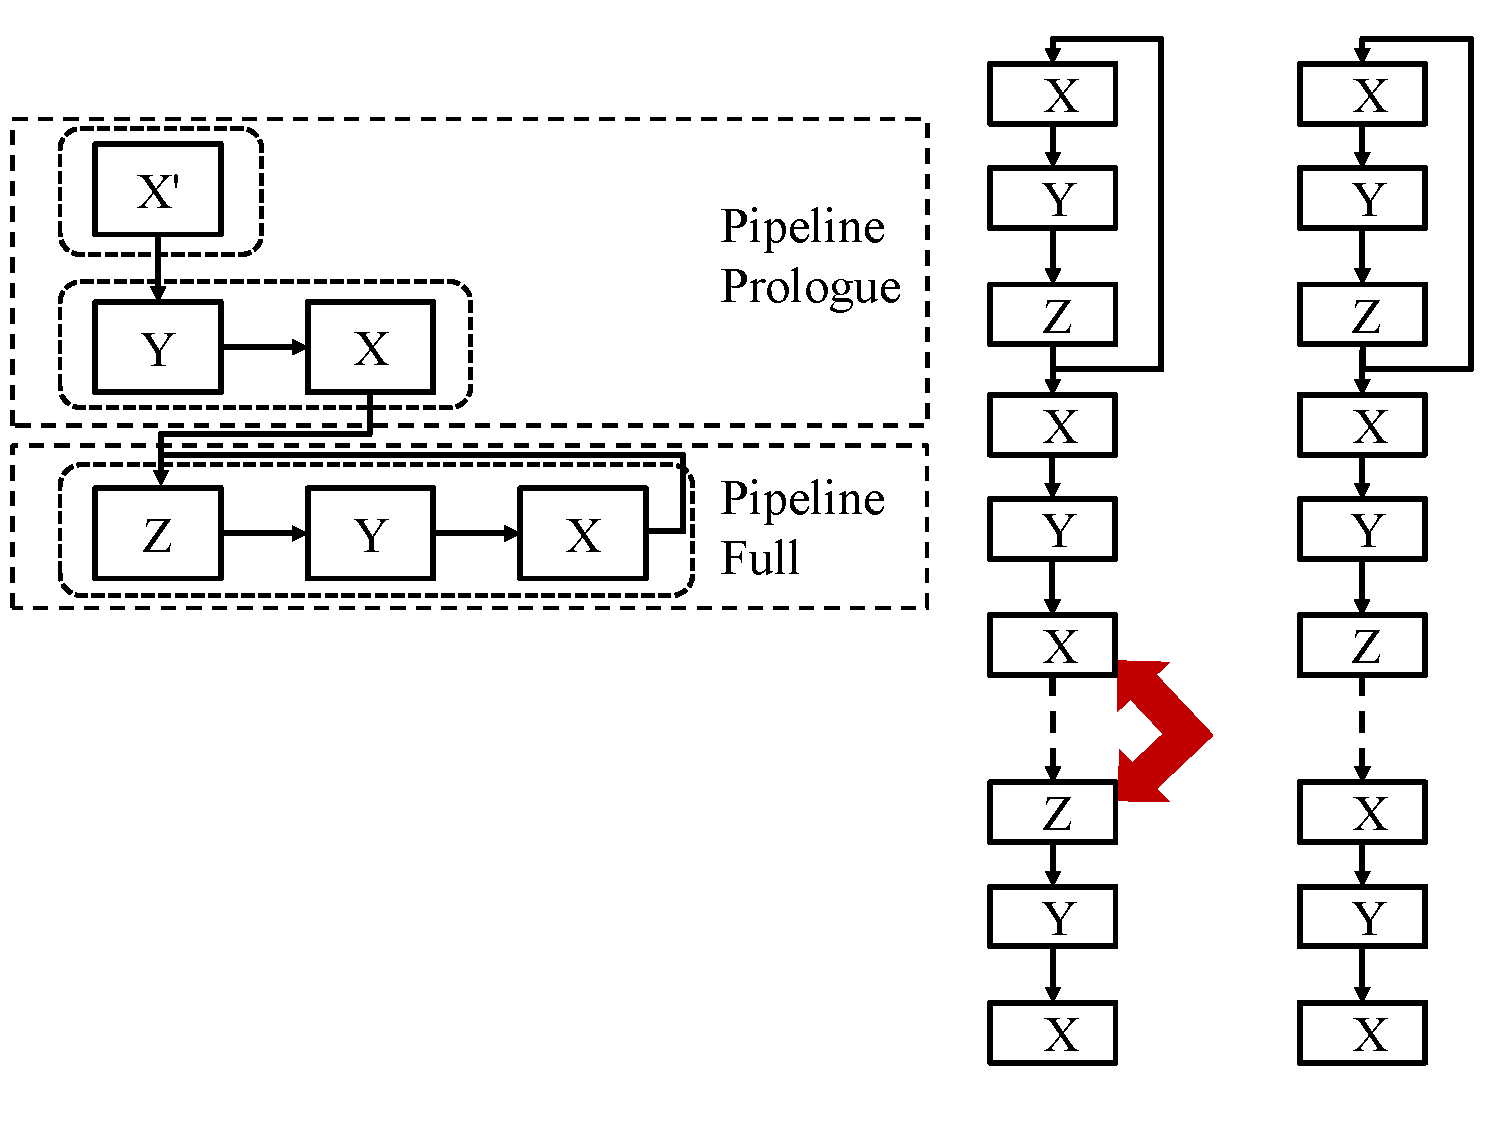
\includegraphics[width=4.25in]{fig-proposal/invariant-inductive-step}
\end{center}
\caption{Invariant Inductive Step}
\label{fig:invariant-inductive-step}
\end{figure}

Although these requirements justify that our correspondence
relation is an invariant, they are used somewhat differently
in the base case (when the number of iterations $k$ of the
pipelined loop is $1$) and inductive step (assume the
invariant holds for $k$ iterations of the pipeline and prove
that it holds for $(k+ 1)$ iterations).  Their usage is
pictorially shown in Figures~\ref{fig:invariant-base-case}
and~\ref{fig:invariant-inductive-step}. For invariant base case where $k$ is
equal to $1$, we commute operations in the loop prologue of
the pipeline (which corresponds to the first iteration after
unrolling) with the loop body. We prove that executing
  pipeline prologue and one pipeline full stage is the same
  as executing $S_{pre}$ followed by a sequence of partially
  completed sequential loop CCDFG. For the inductive step
we work with two consecutive iterations of the loop. Assuming that
  invariant is true for $k$ steps, we prove that executing one pipeline full
  stage on both sides gives us $(k + 1)$ iterations of
  sequantial loop CCDFG followed by partially completed
  sequences as expected.

Our invariant is defined specifically to make the proof
sufficiency straightforward.
Equivalence of CCDFG states of $P$ and $S$ follows from the
invariant by noting that the epilogue $P_{post}$ exactly
constitutes the incomplete scheduling steps of $S$ specified
by the invariant
(cf. Figure~\ref{fig:invariant-implies-correctness}).

\begin{figure}[t!]
\begin{center}
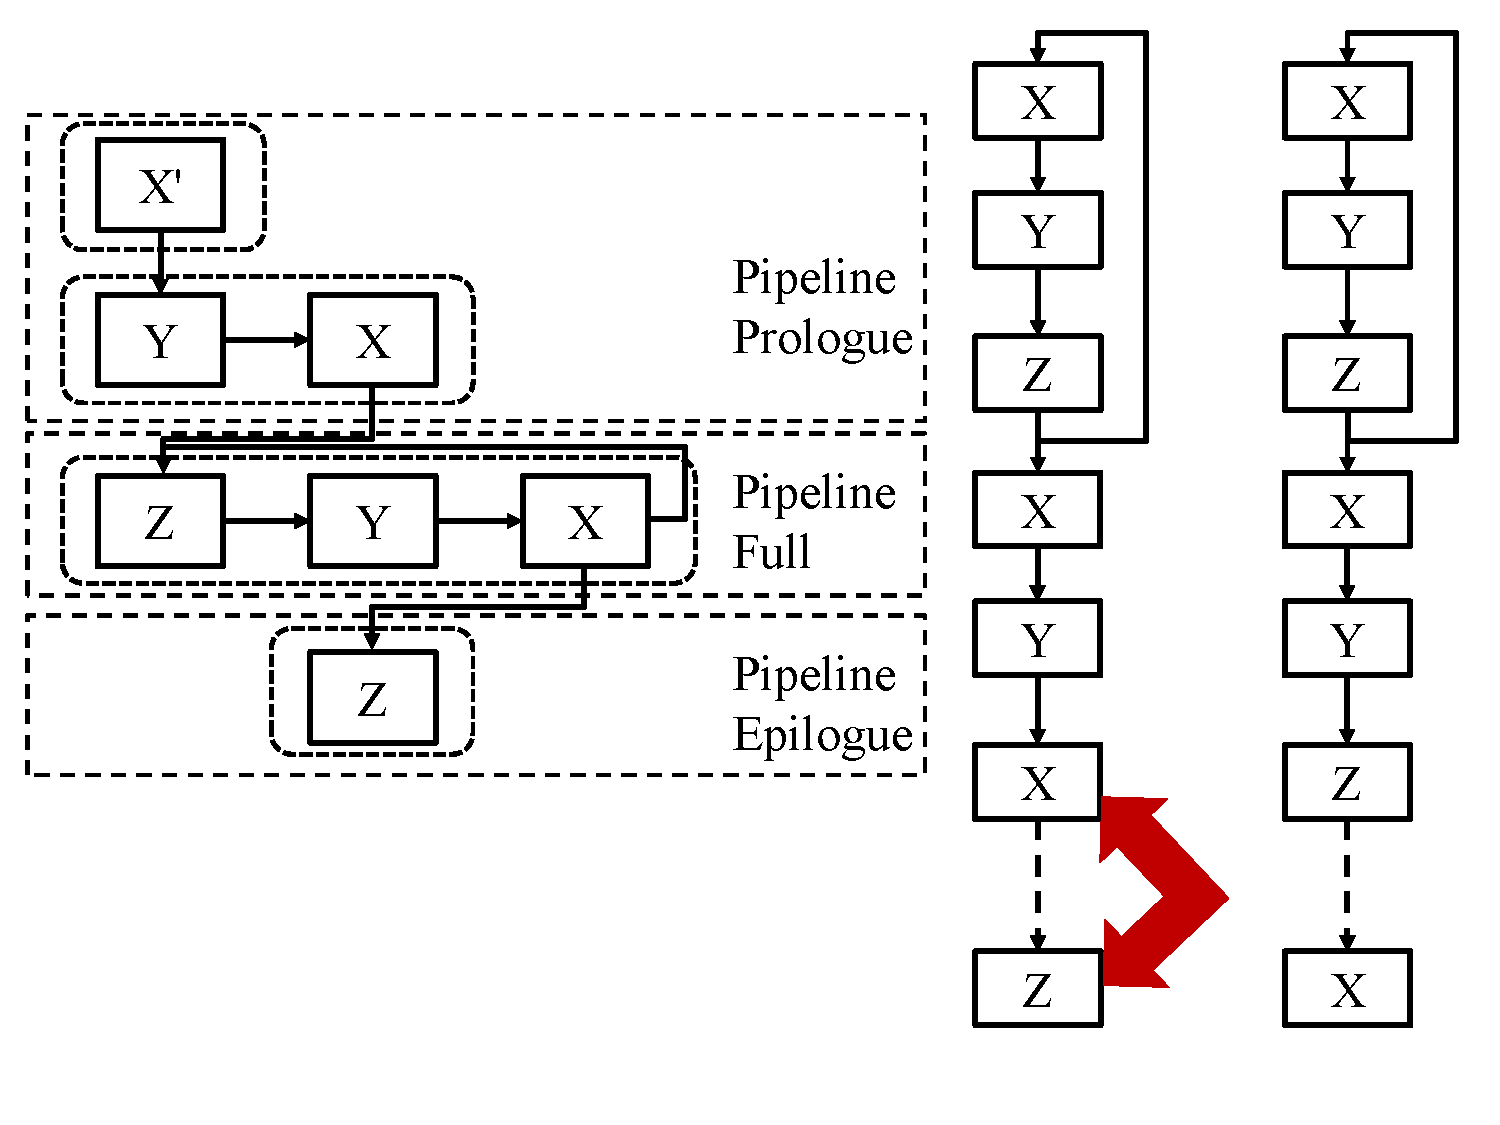
\includegraphics[width=5in]{fig-proposal/invariant-implies-correctness}
\end{center}
\caption{Correctness of invariant implies the correctness statement}
\label{fig:invariant-implies-correctness}
\end{figure}

Our invariant is very different from a typical invariant
used in the verification of pipelined machines (\eg, for
microprocessor pipelines).  We make explicit the
correspondence with the sequential execution.  The key
requirement from a pipeline invariant, \viz, hazard freedom,
is left implicit and arises indirectly as a proof obligation
for invariance of this predicate.  Most microprocessor
pipeline verification work went the other way.  For
instance, Sawada and Hunt's invariant~\cite{sh:pipeline},
expressed through an intermediate structure called MAETT,
``tracks'' the instructions as they pass through different
pipeline stages to ensure that hazards are not introduced.
One difference in our case is that we are not working with a
concrete pipeline with a fixed set of operations but an
algorithm that generates pipelines with an arbitrary
sequence of scheduling steps; a construction like MAETT is
thus not directly applicable.  However, there is a deeper
reason for defining our invariant the way we did.
Suppose we simply unroll the loop in the sequential
design three times, and then use a technique similar to
MAETT to track scheduling steps in this ``unrolled loop
body'' in the pipeline execution.  Unfortunately, this does
not work, because of the back edge.  There is no direct
correlation between this edge and any edge in the sequential
loop.  In fact, it is interesting to observe what its
introduction achieves: completion of one scheduling step in
each of the three partially executed, overlapping loop
iterations.  This suggests that the invariant must
explicitly capture the state of the executions that have
been partially completed during each iteration of the
pipeline ({\em ie}, each traversal of the back edge).

\section{Correctness of Our Algorithm}

The algorithm is essentially built from ground-up using primitives
as shown in Chapter~\ref{sec:pipelining-algorithm}. However, 
apart from proving correctness of each primitive and our key 
invariant, we also need to ensure that the primitive is applied by 
our algorithm properly, {\em i.e.}, the environment
assumptions on which the {\bf correctness of primitive}
depends are maintained appropriately by the algorithm at
the point where the primitive is applied. 
The correctness of each primitive discussed above, entails a
so-called ``assume-guarantee'' reasoning: the primitive is
guaranteed to maintain the desired invariant if and only if
it is applied under certain well-formed conditions.  To use
these correctness statements to verify the algorithm, we
must therefore prove that the algorithm applies each
primitive appropriately, maintaining the well-formedness
condition required for the correctness of the primitive.
Note that verifying this requires an inductive proof
relating the states of the CCDFG $C'$ generated after the
application of the transformation with the original CCDFG
$C$. Note that the induction is non-trivial because
transformations have significant ``global'' effect on a
CCDFG. These include one or more of the following:

\begin{enumerate}
\item Replacing one microstep of $C$ with more than one
  microsteps in $C'$ ({\em e.g.}, $\phi$-elimination), or
\item Interchanging scheduling steps ({\em e.g.},
  interchange), or
\item Changing the variable being read or written in several
  microsteps ({\em e.g.}, shadow register)
\end{enumerate}

The final theorem can be written in ACL2 as 
\small
\begin{verbatim}
(defthm run-random-final-theorem
 (implies (and (well-formed-ccdfg c)
               (well-formed-flow-ccdfg bb sub-bb loc c 
                                       ccdfg-state prev no_seq_steps)
               (equal (list pre loop post) (final-pp c prev interval m)))
               (not (equal (final-pp c prev interval m) "error"))
     (equal (get-final-real-state 
                  (run-ccdfg-random 0 0 0 c ccdfg-state prev no_seq_steps))
            (get-final-real-state 
                  (run-ccdfg-random 0 0 0 (append pre loop post) 
                                              ccdfg-state prev no_pp_steps)))))
\end{verbatim}
\normalsize

The theorem involves several ACL2 functions, \eg, {\tt
well-formed-ccdfg}, \\
{\tt run-ccdfg-random}, etc. Please refer 
our proof scripts for details. Here, we provide a quick overview 
of some of the critical functions in the theorem
below.  

\noindent
$c$ here refers to a sequential loop. We have defined a function {\tt well-formed-ccdfg} 
which imposes restrictions on the structure of the types of loops which can be pipelined. It ensures 
that we have only one conditional branch in $c$ which either points to the next microstep or points to {\tt Exit} somewhere outside $c$. 
It also ensures that we have only one unconditional branch at the end of the loop which points back to the 
beginning of the loop. Moreover, there is only one relevant $\phi$-branch
which is required to handle variables which change value depending on whether previous basic block is outside the loop
or inside. It is required to handle loop carried dependencies as explained before. 
Also, there is only one place of entry and one place of exit in the loop. 
Note that these restrictions are seen in behavioral synthesis tools as well since branches inside/outside the 
loop have already been taken care of before this step using other compiler and scheduling transformations. 
When we reach the pipelining stage, 
we have a {\tt well-defined-ccdfg} loop structure dictated by one conditional and one unconditional branch.

We have also defined a function {\tt well\--formed\--flow\--ccdfg}, which states that starting from the initial basic block {\tt bb}, 
sub-basic-block {\tt sub-bb} and location {\tt loc} of $(0,0,0)$ and an initial state {\tt ccdfg\--state}, if we encounter a branch within $m$ number of steps, then we do not exit {i.e.}, the exit condition variable is not true.  Also, it ensures that the next statement after branch is the next mircostep in order such that we execute the microsteps in order for $m$ number of steps.

The function {\tt run-ccdfg-random} executes a CCDFG starting from the initial basic block {\tt bb}, 
sub-basic-block {\tt sub-bb} and location {\tt loc} of $(0,0,0)$ and an initial state {\tt ccdfg\--state}.

The function {\tt final-pp} applies the pipeline generation algorithm to create the  
list of {\tt pre}, {\tt loop} and {\tt post} as expected. 

Finally, the function {\tt get-final-real-state} removes from the
CCDFG state, all auxiliary variables introduced by
the pipeline generation algorithm itself, leaving only the
variables that correspond to the sequential
CCDFG. Recall that the algorithm has to introduce new variables
  in order to eliminate hazards.  One consequence of this is
  that the new variables so introduced must not conflict
  with any variable subsequently used in the CCDFG.  Since
  we do not have a way to ensure generation of fresh
  variables, this constraint has to be imposed in the
  hypothesis. Also, this function normalizes ``sorts'' the
components in a CCDFG state in a normal form so that the
sequential and pipelined CCDFG states can be compared with
{\tt equal}. 
 
Following is an English paraphrase of the theorem.
  
\begin{quote}  
If the pipeline generation succeeds without error,
executing the pipelined CCDFG (a combination of $pre$, $loop$ and $post$) for $no\_pp\_steps$
generates the same state of the relevant variables as executing the sequential CCDFG $c$ for $no\_seq\_steps$.

\small
\begin{equation}
\begin{split}
no\_seq\_steps &= len S_{1} + (len S * (\ceil{\frac{m}{interval}} - 1)) + len S_{preExit} \\
no\_pp\_steps &= len P_{pre} + (len P_{loop} * k) + len P_{post}
\end{split}
\end{equation}

%\ceil{n / interval}) 

%no\_pp\_steps &= (len P_{pre}) + ((len P_{loop}) * k) + (len P_{post})
\normalsize

\end{quote}

We can take each stage one by one to understand the complexity involved in 
verifying the algorithm as a whole, over and above the verification of 
individual primitives.

\begin{enumerate}
\item \textbf{Remove Branches}: In the $Remove Branches$ stage, which is the first stage of pipelining algorithm, we have to create a correspondence between randomly executing a CCDFG with branches using basic-block, sub-basic-block and location with executing a CCDFG in sequence without a conditional and unconditional branch as shown in Figure~\ref{fig:proof-remove-branches}. This is similar to branch primitive, but since we have a non-streamlined run on one side and a steamlined sequential run on the other side, there are theorems involved with finding the next microstep randomly and proving that it is same as the next microstep in streamlined order. We also need to prove that the applicaton of branch primitive is correct. After this step and for all the subsequent steps, we need to show that there are no relevant branches in CCDFG.
                                             
\begin{figure}[t!]
\begin{center}
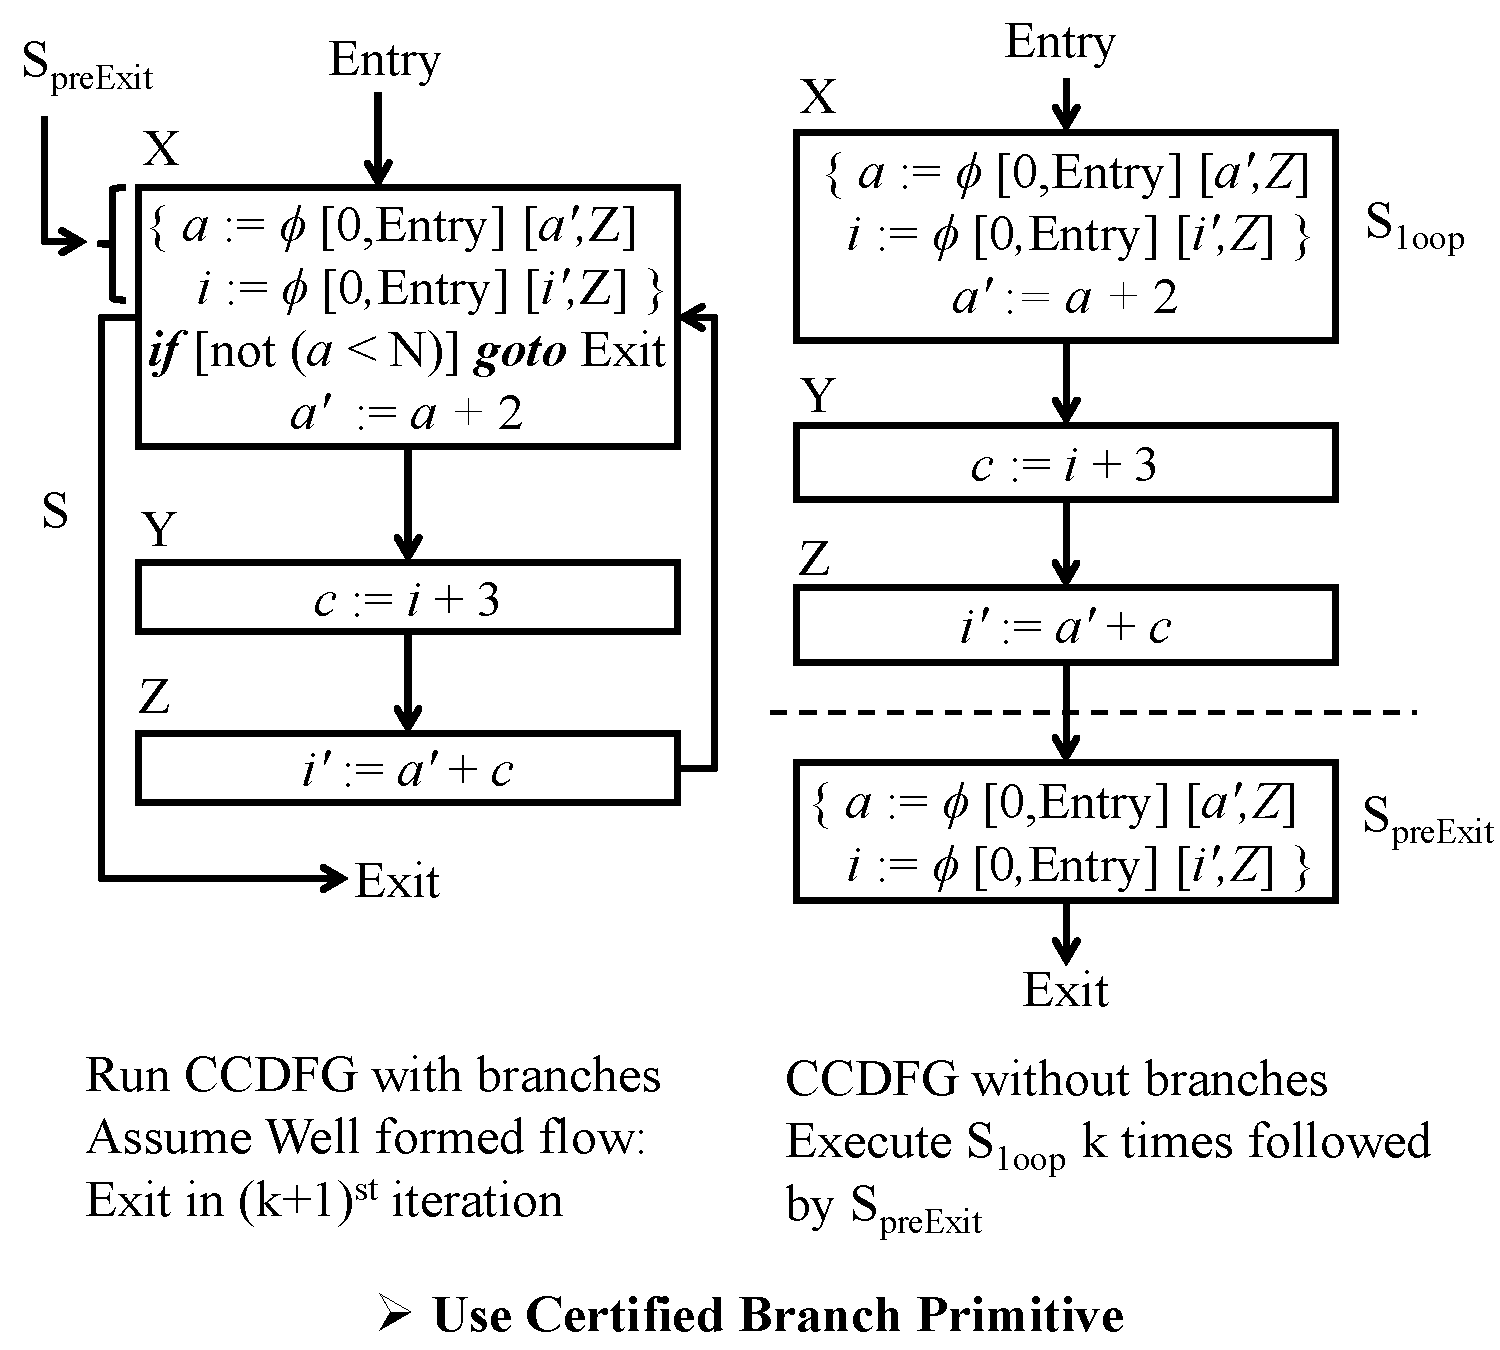
\includegraphics[height=3.5in]{fig-proposal/proof-remove-branches}
\end{center}
\caption{Proof Sketch for Remove Branches Stage}
\label{fig:proof-remove-branches}
\end{figure}

\item \textbf{Unroll Loop Once}: This step unrolls the loop by one as explained before. The proof uses induction along the number of iterations.

\item \textbf{$\phi$-to-assign}: In the $\phi$-to-assign stage, we replace one microstep of $C$ with more than one microsteps in $C'$
as shown in Figure~\ref{fig:proof-after-phi}. 
In addition to inductively reasoning about application of a primitive in entire CCDFG, we also have to ensure
that addition of new microsteps does not affect the basic structure of the CCDFG. These well-formed-conditions need to be maintained at each step to ensure that the primitives can be applied.



\begin{figure}[H]
\begin{center}
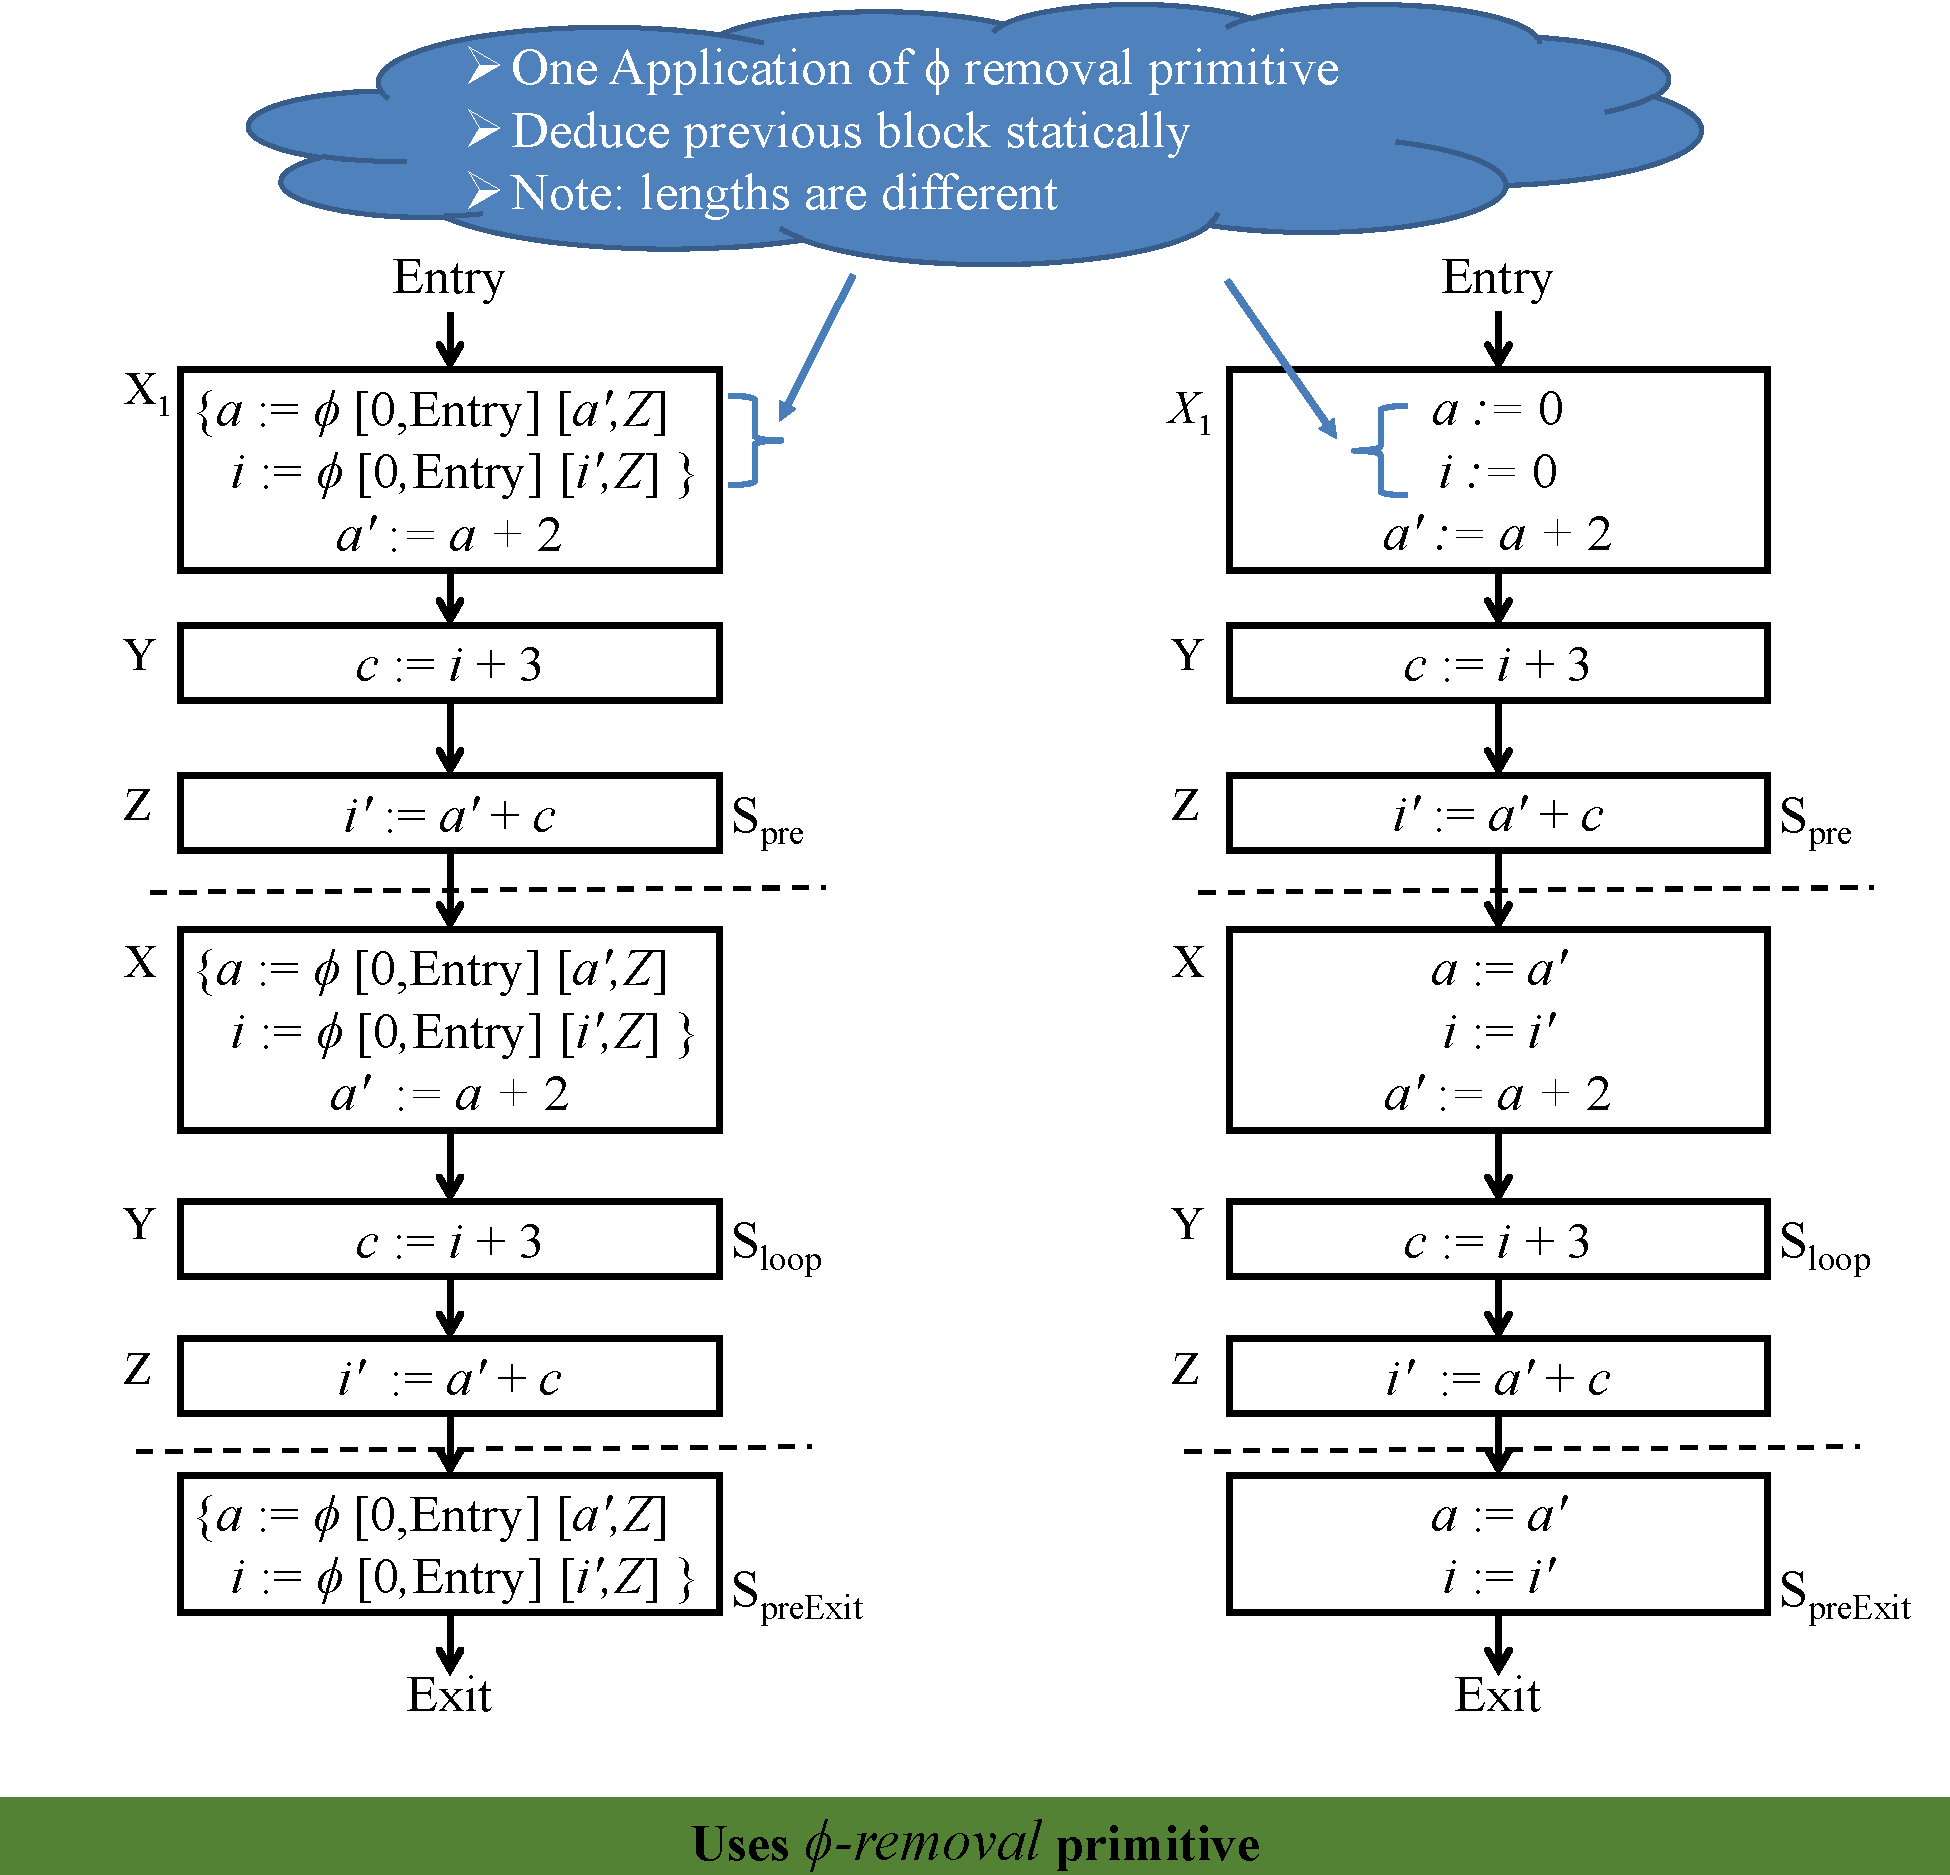
\includegraphics[width=5.5in]{fig-proposal/proof-after-phi}
\end{center}
\caption{Proof Sketch for $\phi$-to-assign Step}
\label{fig:proof-after-phi}
\end{figure}

The upshot is that an inductive theorem relating $C$ and $C'$ must be strong enough to 
comprehend the global effects. For instance, an inductive statement showing the
correctness of $\phi$-elimination must account for the fact
that the number of microsteps of $C$ is different from that
of $C'$.  Thus an execution of $C$ for $n$ microsteps must
correspond to an execution of $C'$ for a different number
$m$ of microsteps, where the number $m$ is a function of $n$
and the structures of $C$ and $C'$; the statement of the
correctness of $\phi$-elimination must characterize the
value of $m$ precisely, perhaps defining functions that
statically and symbolically execute $C$ and $C'$, in order
to be provable by induction.  Furthermore the functions so
introduced for static symbolic execution must themselves be
proven correct.



\item {\textbf {Data Propagation}} : In the data propagation stage, the first step involves identifying 
the appropriate statements that cause conflict and applying interchange primitive multiple times 
to move the microstep to the beginning of the loop. We need to make sure that the conditions under which
interchange primitive can be further applied are maintained after each application.
 
The second step involves moving the microstep into the previous iteration. 
It requies removing the microstep, referred as $mstep$ from beginning of $S_{loop}$ and adding it to end of $S_{loop}$. 
Also, $mstep$ is added in $S_{pre}$ and removed 
from $S_{preExit}$. The proof of this step requires non-trivial induction as explained in Figures~\ref{fig:proof-after-data-propagation-basecase} and ~\ref{fig:proof-after-inductive-step}. 
These stages need to be
repeated for as many variables as are in conflict. 

\item \textbf{Shadow-register}: Recall that shadow register step adds many more new statements to assign temporary values to 
new shadow variables. The addition of new microsteps means that in addition to inductively reasoning about application of a primitive in entire CCDFG, we also have to ensure that basic structure of the CCDFG is maintained. Moreover, we need to reason about read and write of 
variables across a number of microsteps. The proof is analogous to the proof of shadow-register primitive. However, the primitive is applied multiple times based on the variabes which are causing conflict. This gets tricky as after application of one primitive, there are new variables introduced and we can only claim that the relevant variables have same value.

\begin{figure}[t!]
\begin{center}
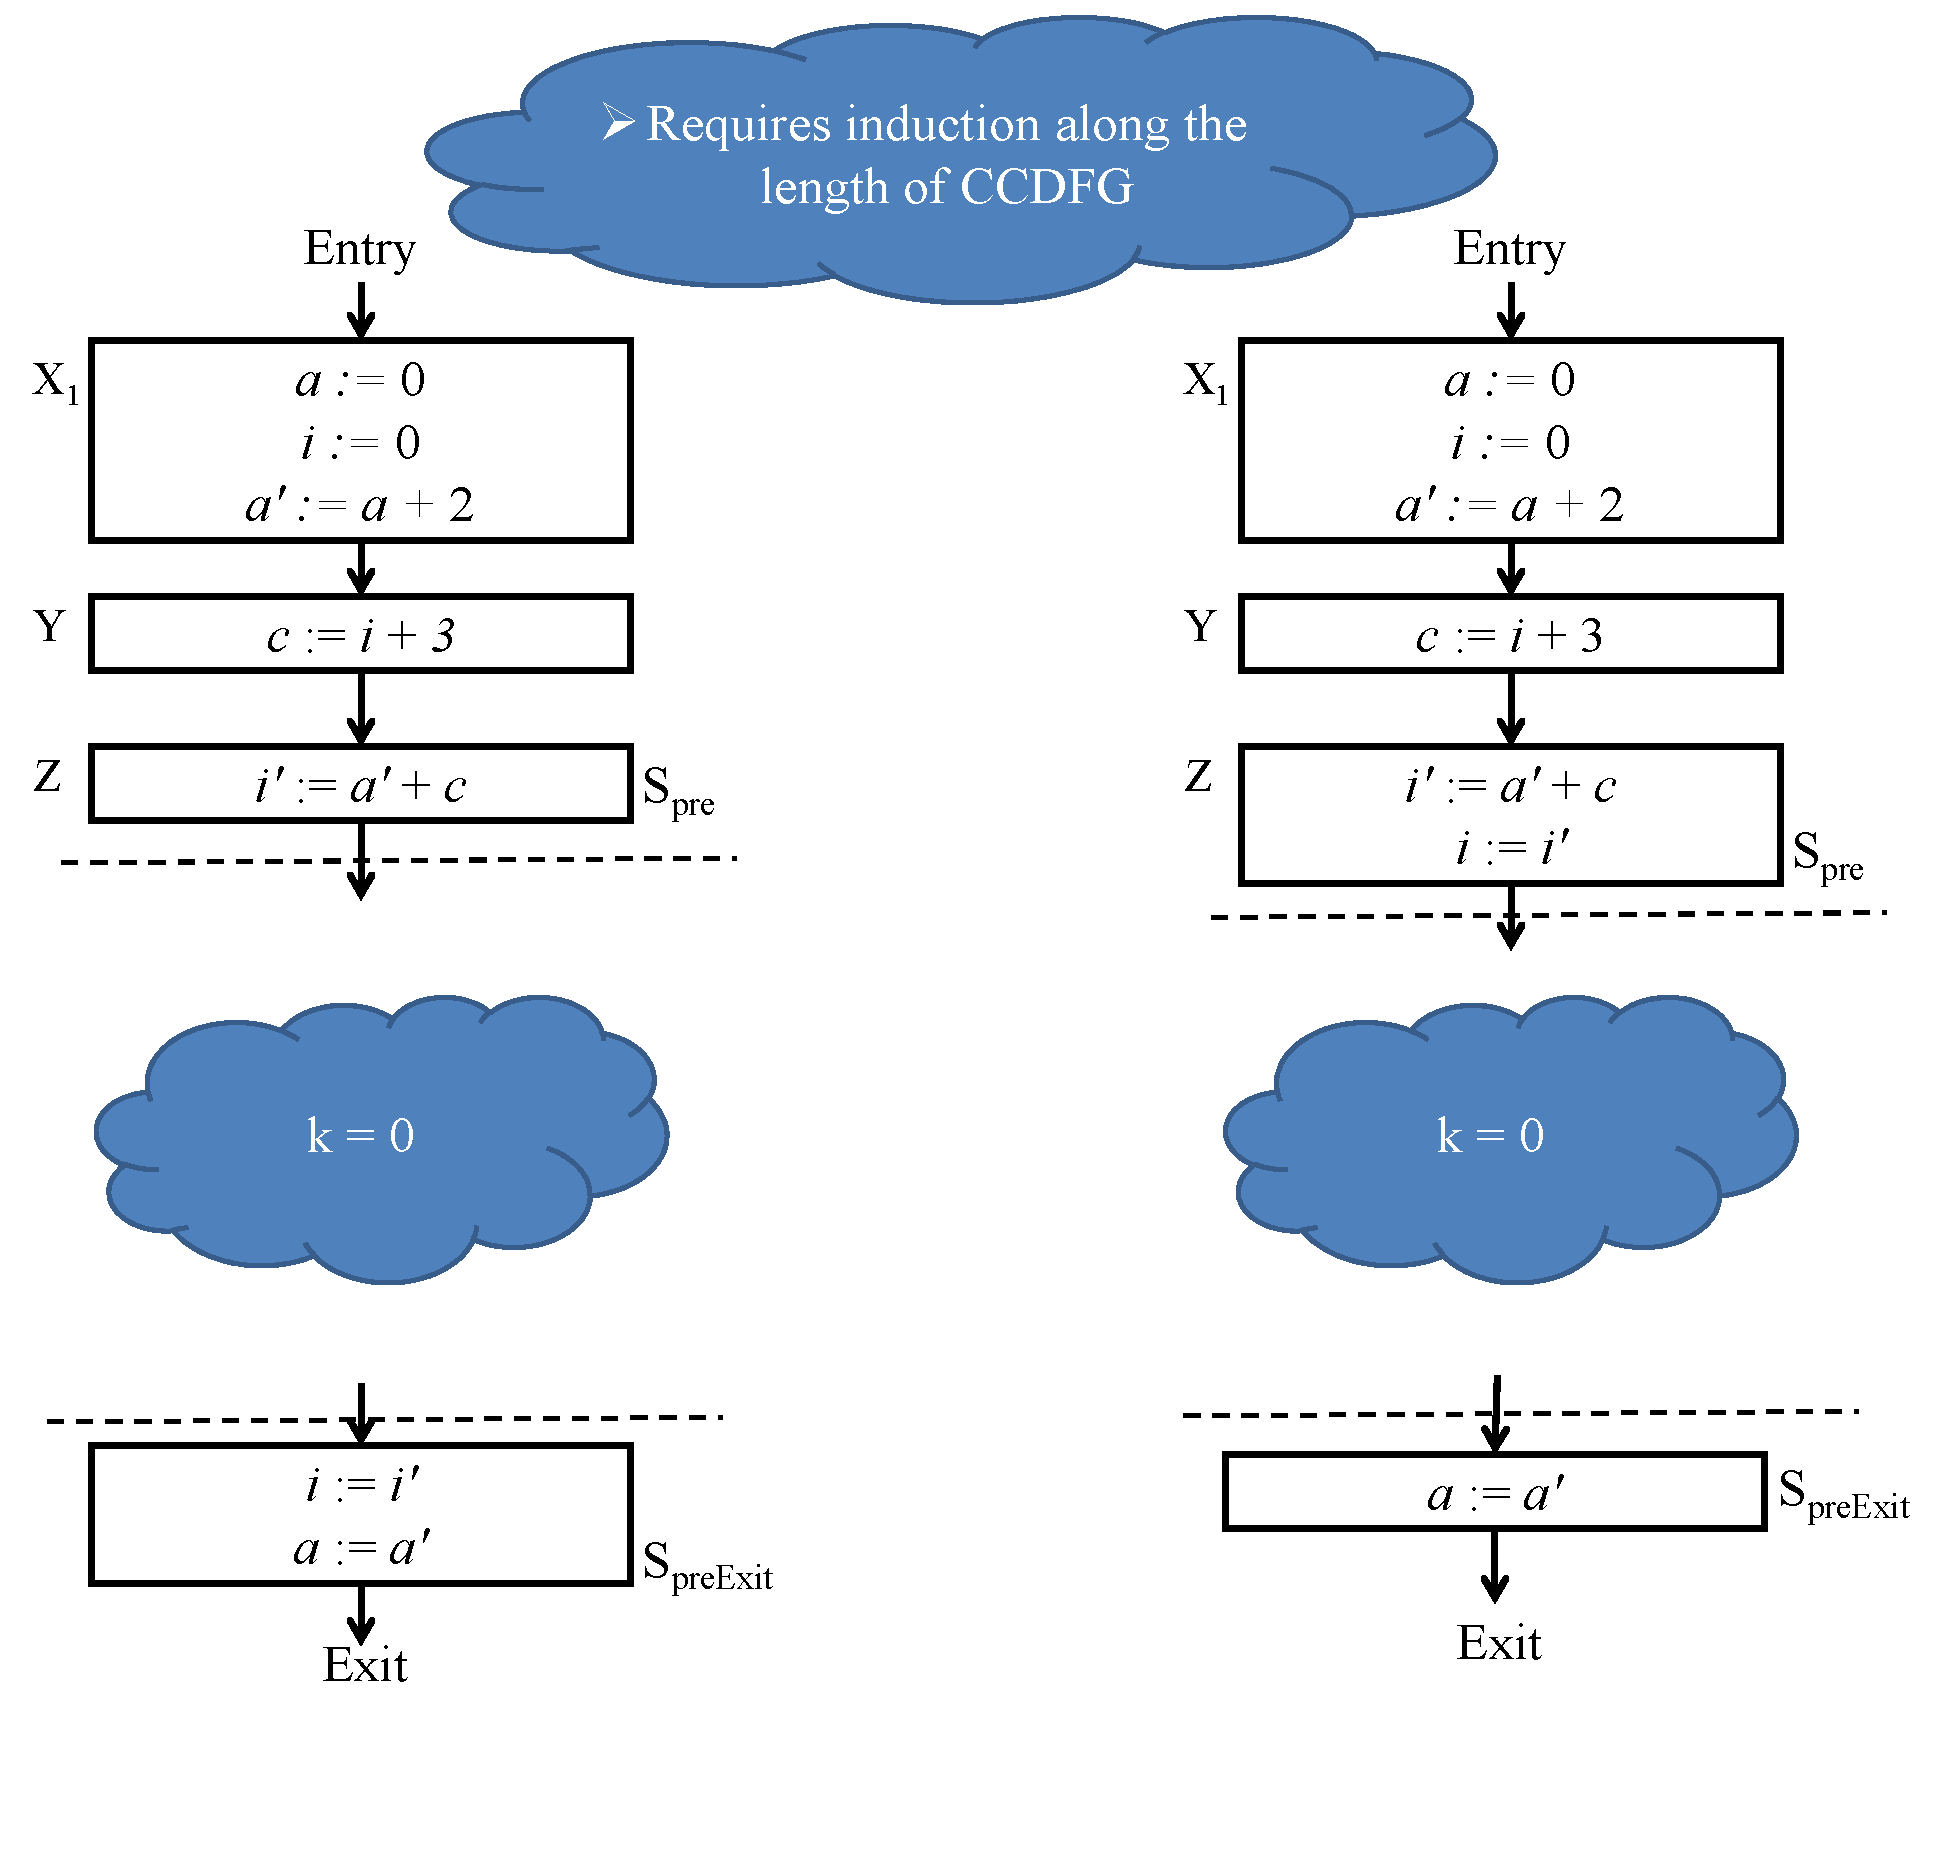
\includegraphics[width=5.5in]{fig-proposal/proof-after-data-propagation-basecase}
\end{center}
\caption{Proof Sketch for Data Propagation Step Base Case}
\label{fig:proof-after-data-propagation-basecase}
\end{figure}

\clearpage
\begin{sidewaysfigure}[t!]
\begin{center}
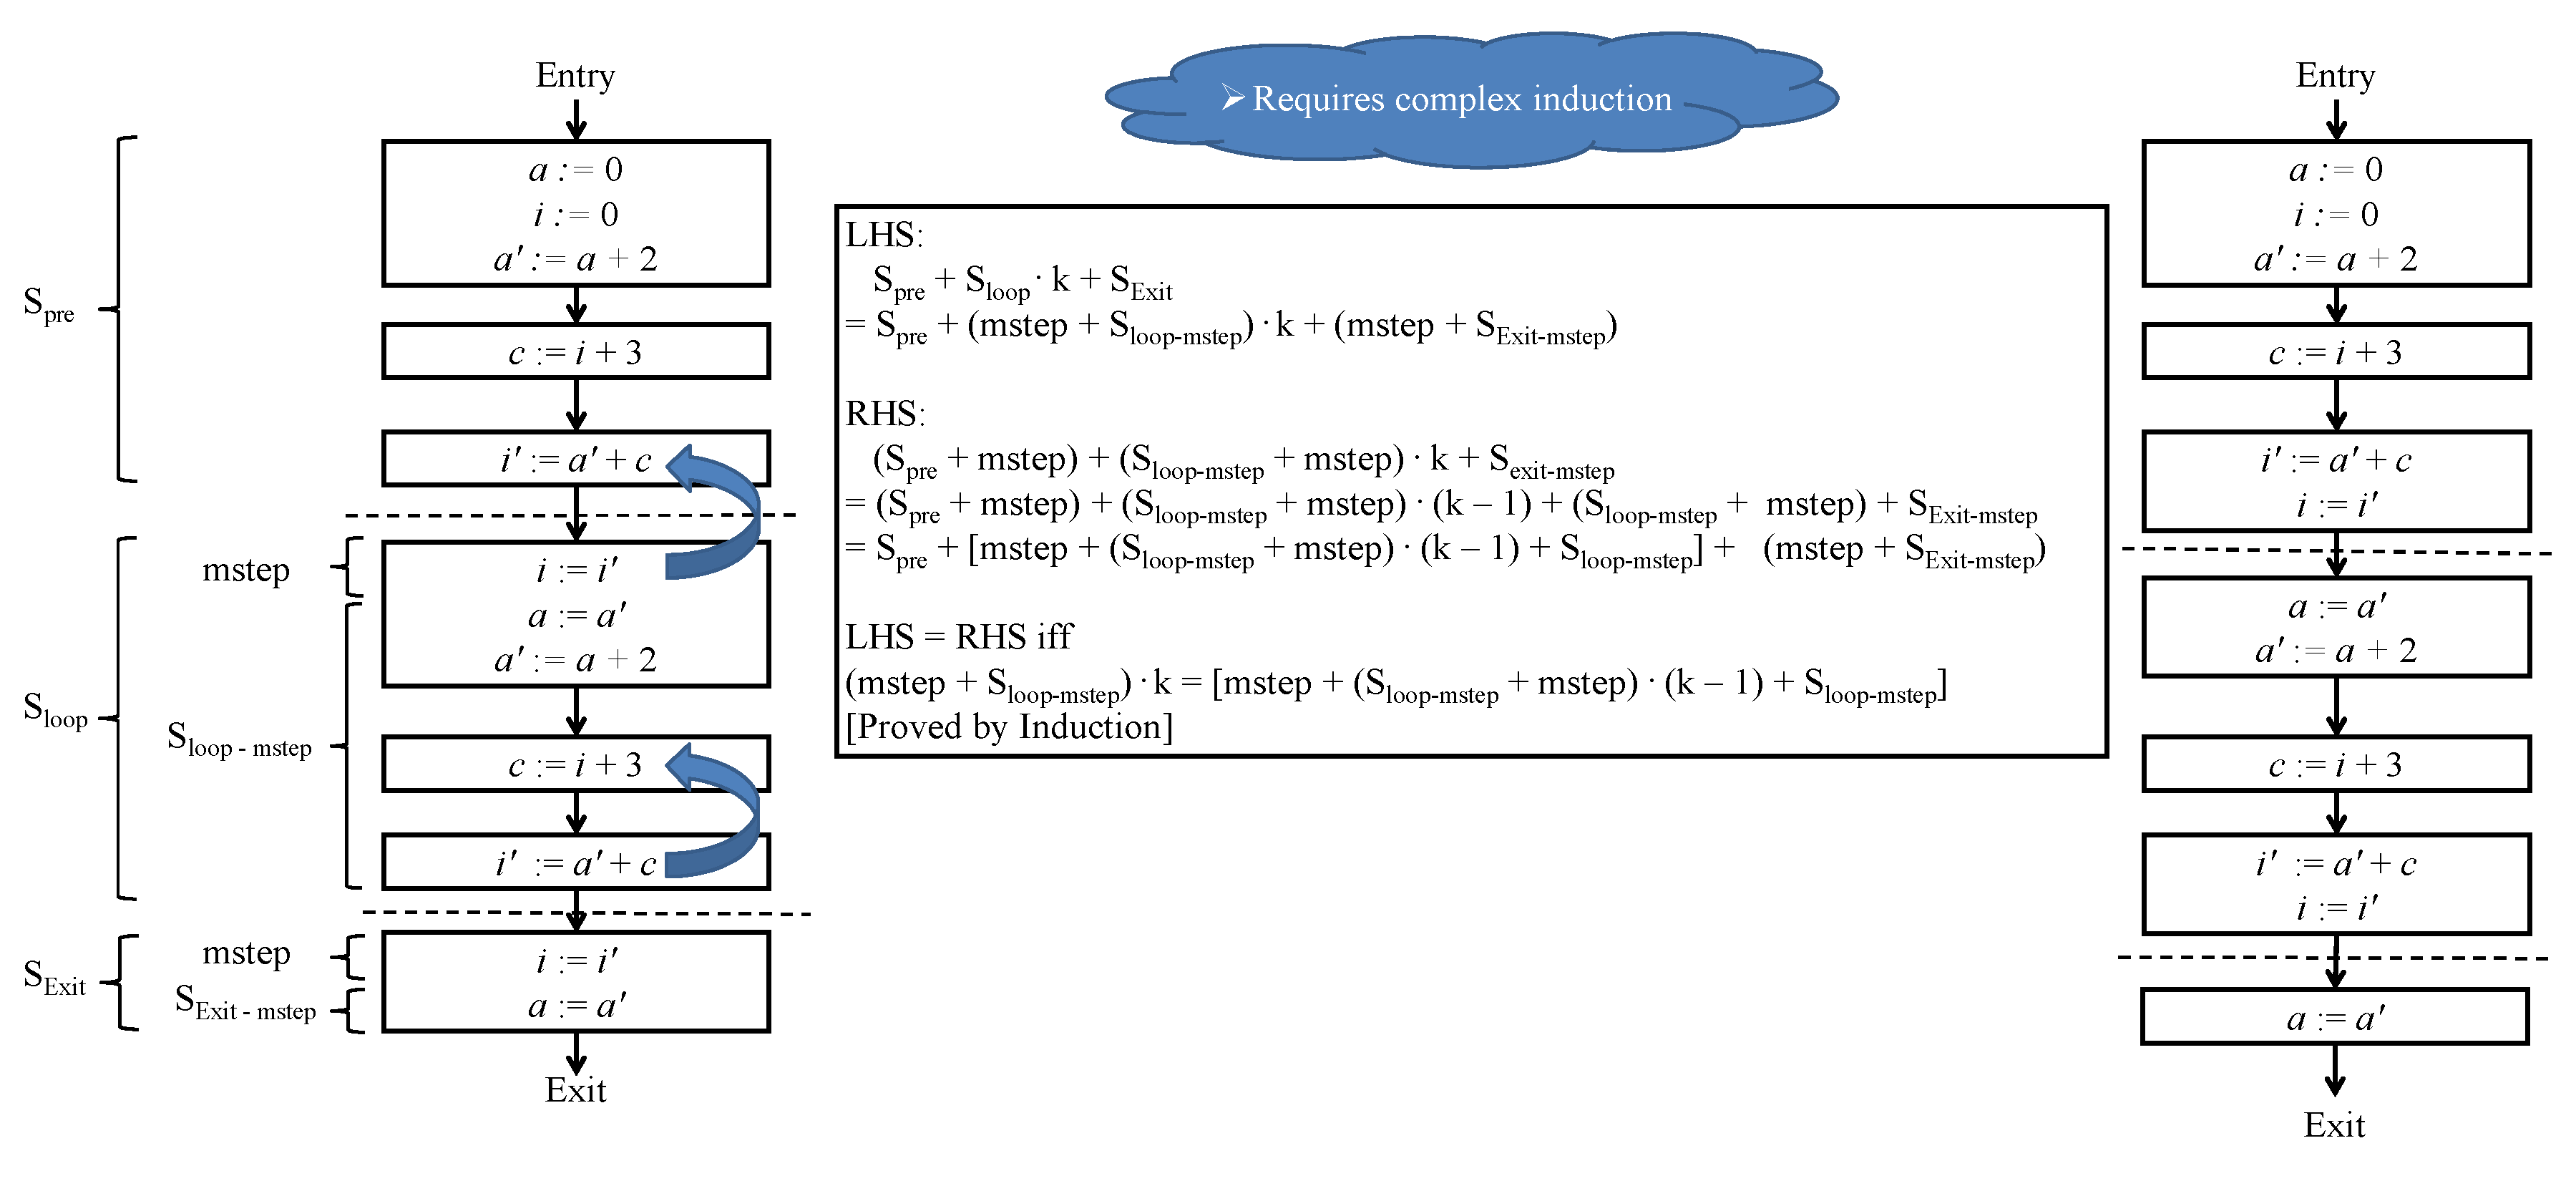
\includegraphics[height=4in]{fig-proposal/proof-after-inductive-step}
\end{center}
\caption{Proof Sketch for Data Propagation Step}
\label{fig:proof-after-inductive-step}
\end{sidewaysfigure}
\clearpage
 
\item \textbf{Superstep-construction}: This step requies proof of invariant and multiple applications of interchange primitive as explained earlier. 

\item \textbf{AddBranches}: The proof required is the reverse of branch-primitive. However, a key requirement is that branch-primitive can be applied only when we have a {\tt well-formed-ccdfg}, so we need to ensure that the structure of the $loop$ before adding branches is such that the final $loop$ in the pipelined CCDFG is indeed a {\tt well-formed-ccdfg}.  

\end{enumerate}

\section{Lessons from Previous False Starts}

Before we came up with our approach of building a pipelining
algorithm using a framework of certified pipelining primitives,
we tried a few other intuitive approaches.
From each false start, we were able to learn something valuable.

In our initial approach we had decided to simplify the problem
by ignoring the back edge and proving the correspondence
between an unrolled loop and the pipeline.
Only after substantially completing this proof and in
attempting to extend it to the pipeline with the back edge
did we realize that the extension does not work. So, we came up with a key
invariant to deal with this problem.

Also, we attempted initially to stick to the previously proposed algorithm
and try to prove that the execution of the input is equal to the execution
of the output for the complete algorithm. To do that, we need to claim that
the output pipeline does not introduce any data hazards.
Hazard freedom entails showing the
following. ``Suppose a variable $v$ is written by a
scheduling step $S$ and read subsequently by a scheduling
step $S'$ in the sequential CCDFG.  Then in the pipelined
CCDFG, there is no scheduling step $P$ that writes $v$ and
is executed between $S$ and $S'$.''  Originally, we defined
this notion directly for each variable, \viz, with a
function that statically analyzes the CCDFG to identify the
range of scheduling steps between a write and subsequent
read of each variable.  However, this does not
work.  For example, proving this property for variable $x$
may require a similar property to hold for another variable
$y$ (perhaps because $x$ is assigned an expression involving
$y$).  But the range of scheduling steps in which $x$ and
$y$ are read and written are different, and the extension of
the property to all the variables cannot be easily specified
by an invariant for any specific scheduling step. When we realized
the challenges involved in proving the complete algorithm,
it led us to propose our framework of pipelining primitives.
Also, our current approach succinctly captures an ``on-track property'',
\viz, that the
state after $k$ pipeline iterations is equivalent to partial
execution of a certain number of iterations in the
sequential CCDFG (in addition to completion of $k'$
iterations) which avoids this problem and can indeed be
specified as an invariant.

